\subsection{Kravgrunnlag og prosjektlogg}
% Sett inn gjeldende oppgavegrunnlag og relevante avklaringer.
\subsection{Risikovurdering}
\label{app:risiko}
Risiko vurderes som produktet av sannsynlighet og påvirkning, begge på en skala fra 1 til 5, og klassifiseres etter risikomatrisen i tabell~\ref{tab:risikomatrise}. Risikoen er delt i personskade ved det praktiske arbeidet og forhold som kan hindre gjennomføringen av prosjektet.

% Celler i risikomatrisen: \riskcell{farge}{nivå}{poeng}
\newcommand{\riskcell}[3]{\cellcolor{#1}\textbf{#2}\newline\textbf{#3}}
% Risikopoeng farget etter nivå i risikomatrisen: \riskscore{poeng}
\newcommand{\riskscore}[1]{%
    \ifnum#1>14 \cellcolor{riskextreme}\else
    \ifnum#1>7 \cellcolor{riskhigh}\else
    \ifnum#1>3 \cellcolor{riskmoderate}\else
    \cellcolor{risklow}\fi\fi\fi #1}
% Kolonner for risikotabellene; hendelsen brytes over flere linjer ved behov
\newcolumntype{E}{>{\centering\arraybackslash}m{6.4cm}}
\begin{table}[H]
    \centering
    \caption{Risikomatrise}
    \label{tab:risikomatrise}
    \small
    \renewcommand{\arraystretch}{1.5}
    \begin{tabular}{|c|>{\centering\arraybackslash}m{3.0cm}|*{5}{>{\centering\arraybackslash}m{1.6cm}|}}
        \hline
        \multicolumn{2}{|c|}{} & \multicolumn{5}{c|}{\textbf{Påvirkning}} \\
        \cline{3-7}
        \multicolumn{2}{|c|}{} & \textbf{Lav}\newline\textbf{1} & \textbf{Liten}\newline\textbf{2} & \textbf{Moderat}\newline\textbf{3} & \textbf{Høy}\newline\textbf{4} & \textbf{Alvorlig}\newline\textbf{5} \\
        \hline
        & \textbf{Svært sannsynlig}\newline\textbf{5} & \riskcell{riskmoderate}{Moderat}{5} & \riskcell{riskhigh}{Høy}{10} & \riskcell{riskextreme}{Ekstrem}{15} & \riskcell{riskextreme}{Ekstrem}{20} & \riskcell{riskextreme}{Ekstrem}{25} \\
        \cline{2-7}
        & \textbf{Sannsynlig}\newline\textbf{4} & \riskcell{riskmoderate}{Moderat}{4} & \riskcell{riskhigh}{Høy}{8} & \riskcell{riskhigh}{Høy}{12} & \riskcell{riskextreme}{Ekstrem}{16} & \riskcell{riskextreme}{Ekstrem}{20} \\
        \cline{2-7}
        & \textbf{Nøytral}\newline\textbf{3} & \riskcell{risklow}{Lav}{3} & \riskcell{riskmoderate}{Moderat}{6} & \riskcell{riskhigh}{Høy}{9} & \riskcell{riskhigh}{Høy}{12} & \riskcell{riskextreme}{Ekstrem}{15} \\
        \cline{2-7}
        & \textbf{Lite sannsynlig}\newline\textbf{2} & \riskcell{risklow}{Lav}{2} & \riskcell{riskmoderate}{Moderat}{4} & \riskcell{riskmoderate}{Moderat}{6} & \riskcell{riskhigh}{Høy}{8} & \riskcell{riskhigh}{Høy}{10} \\
        \cline{2-7}
        \multirow{-10}{*}{\rotatebox[origin=c]{90}{\textbf{Sannsynlighet}}} & \textbf{Sjelden}\newline\textbf{1} & \riskcell{risklow}{Lav}{1} & \riskcell{risklow}{Lav}{2} & \riskcell{risklow}{Lav}{3} & \riskcell{riskmoderate}{Moderat}{4} & \riskcell{riskmoderate}{Moderat}{5} \\
        \hline
    \end{tabular}
\end{table}

\paragraph{Personskade}
Tabell~\ref{tab:risiko-arbeid} viser HMS-relatert risiko knyttet til det praktiske arbeidet.

\begin{table}[H]
    \centering
    \caption{Vurdering av potensielle skadefaktorer}
    \label{tab:risiko-arbeid}
    \small
    \begin{tabular}{|c|E|c|c|c|}
        \hline
        nr & \textbf{Potensielle hendelser} & \textbf{Sannsynlighet} & \textbf{Påvirkning} & \textbf{Risikopoeng} \\
        \hline
        \textbf{1.} & Skader fra bruk av dreiebenk & 3 & 4 & \riskscore{12} \\
        \hline
        \textbf{2.} & Brannskade ved sveising & 2 & 5 & \riskscore{10} \\
        \hline
        \textbf{3.} & Brannskade av 3D-printer & 1 & 2 & \riskscore{2} \\
        \hline
        \textbf{4.} & Klemmer finger i bilmekanisme & 1 & 3 & \riskscore{3} \\
        \hline
        \textbf{5.} & Skade av verktøy (Ubåten) & 2 & 3 & \riskscore{6} \\
        \hline
    \end{tabular}
\end{table}

Tiltak for å redusere risiko for personskade, nummerert etter hendelsene i tabell~\ref{tab:risiko-arbeid}:
\begin{enumerate}
    \item \textbf{Dreiebenk:} Få opplæring før bruk og følg verkstedets instrukser. Bruk vernebriller, unngå løse klær, smykker og løst hår, og forlat aldri maskinen mens den går.
    \item \textbf{Sveising:} Følg alle instrukser knyttet til bruk av sveiseapparat. Blant annet: ikke bruk plagg med lange ermer, bruk påbudt sikkerhetsutstyr til enhver tid og ha brannslukningsapparat tilgjengelig.
    \item \textbf{3D-printer:} Ikke ta på dysen eller printplaten før printen er ferdig og har kjølt seg ned.
    \item \textbf{Bilmekanismen:} Kontroller innfesting før opptrekk, og hold hender og løse gjenstander unna roterende deler.
    \item \textbf{Verktøy i Ubåten:} Utvis sunn varsomhet, sett av god tid til oppgavene som skal utføres, bruk nødvendig verneutstyr og følg verkstedets sikkerhetsrutiner.
\end{enumerate}

\paragraph{Gjennomføring av prosjektet}
Tabell~\ref{tab:risiko-gjennomforing} viser hendelser som kan forsinke eller hindre prosjektet.

\begin{table}[H]
    \centering
    \caption{Potensielle hendelser under gjennomføring av prosjektet}
    \label{tab:risiko-gjennomforing}
    \small
    \begin{tabular}{|c|E|c|c|c|}
        \hline
        nr & \textbf{Potensielle hendelser} & \textbf{Sannsynlighet} & \textbf{Påvirkning} & \textbf{Risikopoeng} \\
        \hline
        \textbf{1.} & 3D-print feiler & 4 & 2 & \riskscore{8} \\
        \hline
        \textbf{2.} & Gruppemedlem blir syk & 1 & 3 & \riskscore{3} \\
        \hline
        \textbf{3.} & Konsept fungerer ikke & 3 & 3 & \riskscore{9} \\
        \hline
        \textbf{4.} & Deler blir skadet & 4 & 3 & \riskscore{12} \\
        \hline
        \textbf{5.} & Utdelte komponenter har avvikende dimensjoner eller skjevheter som må rettes & 2 & 3 & \riskscore{6} \\
        \hline
    \end{tabular}
\end{table}
Påvirkningen for hendelse 4 i tabell~\ref{tab:risiko-gjennomforing} avhenger av hvilken del som blir skadet. 3D-printede deler er lette å bytte ut, mens for eksempel svinghjulet er vanskeligere å erstatte.

Tiltak for å redusere påvirkning på prosjektets fremgang, nummerert etter hendelsene i tabell~\ref{tab:risiko-gjennomforing}:
\begin{enumerate}
    \item \textbf{Feilet 3D-print:} Rengjør printplaten med sprit før utskrift og følg med på minst de to første lagene. Start utskrift av kritiske deler tidlig, slik at det er tid til å printe på nytt.
    \item \textbf{Sykdom:} Gruppen består bare av ett medlem. Ved langvarig sykdom må evt. veileder kontaktes. 
    \item \textbf{Konseptet fungerer ikke:} Test delsystemer tidlig, allerede mens designet utvikles, og unngå store, drastiske designendringer sent i prosjektet.
    \item \textbf{Skadde deler:} Ha reservedeler av 3D-printede komponenter og ferdige printfiler klare, slik at skadde deler kan erstattes raskt. Deler som er vanskelige å erstatte, som svinghjulet, håndteres og lagres forsiktig.
    \item \textbf{Avvikende utdelte komponenter:} Mål opp utdelte komponenter ved mottak, kontroller kritiske mål og test delsystemer før full montering, slik at skjevheter og dårlig passform oppdages tidlig.
\end{enumerate}
Generelle tiltak som ikke knytter seg til én enkelt hendelse:
\begin{itemize}
    \item Leveringstid og verkstedtilgang: avklar kritiske deler og bestill eller reserver tid tidlig.
    \item Varierende opptrekk og underlag: standardiser testprosedyren og registrer avvik.
\end{itemize}

\clearpage
\subsection{Arbeidstegninger og deleliste}
\label{app:tegninger}

\begin{sidewaysfigure}
    \centering
    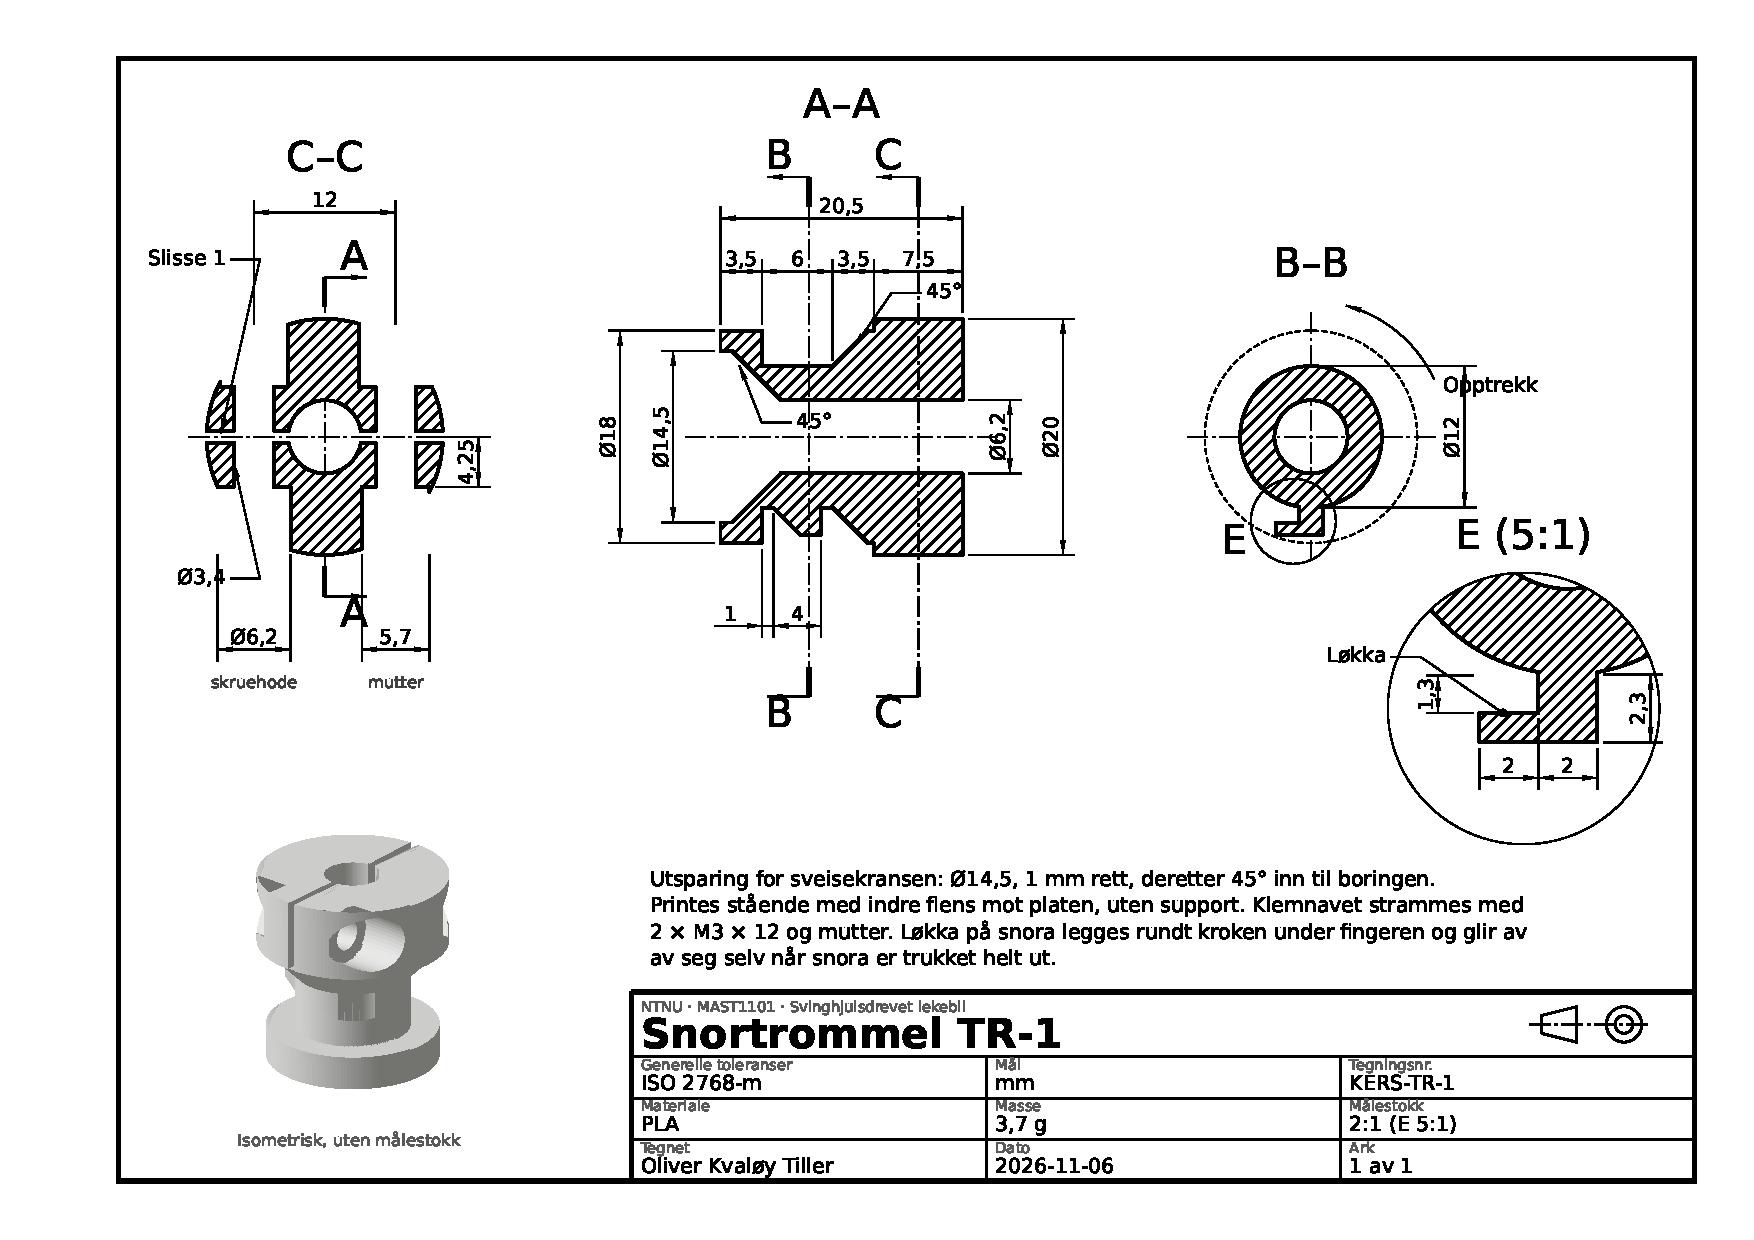
\includegraphics[width=\textheight]{Images/Tegninger/TR-1.pdf}
    \caption{Maskintegning av snortrommelen med Ø12-kjerne. Snitt A--A langs aksen, C--C gjennom klemskruene, B--B gjennom kroken og detalj E av kroken.}
    \label{fig:snortrommel}
\end{sidewaysfigure}

\begin{sidewaysfigure}
    \centering
    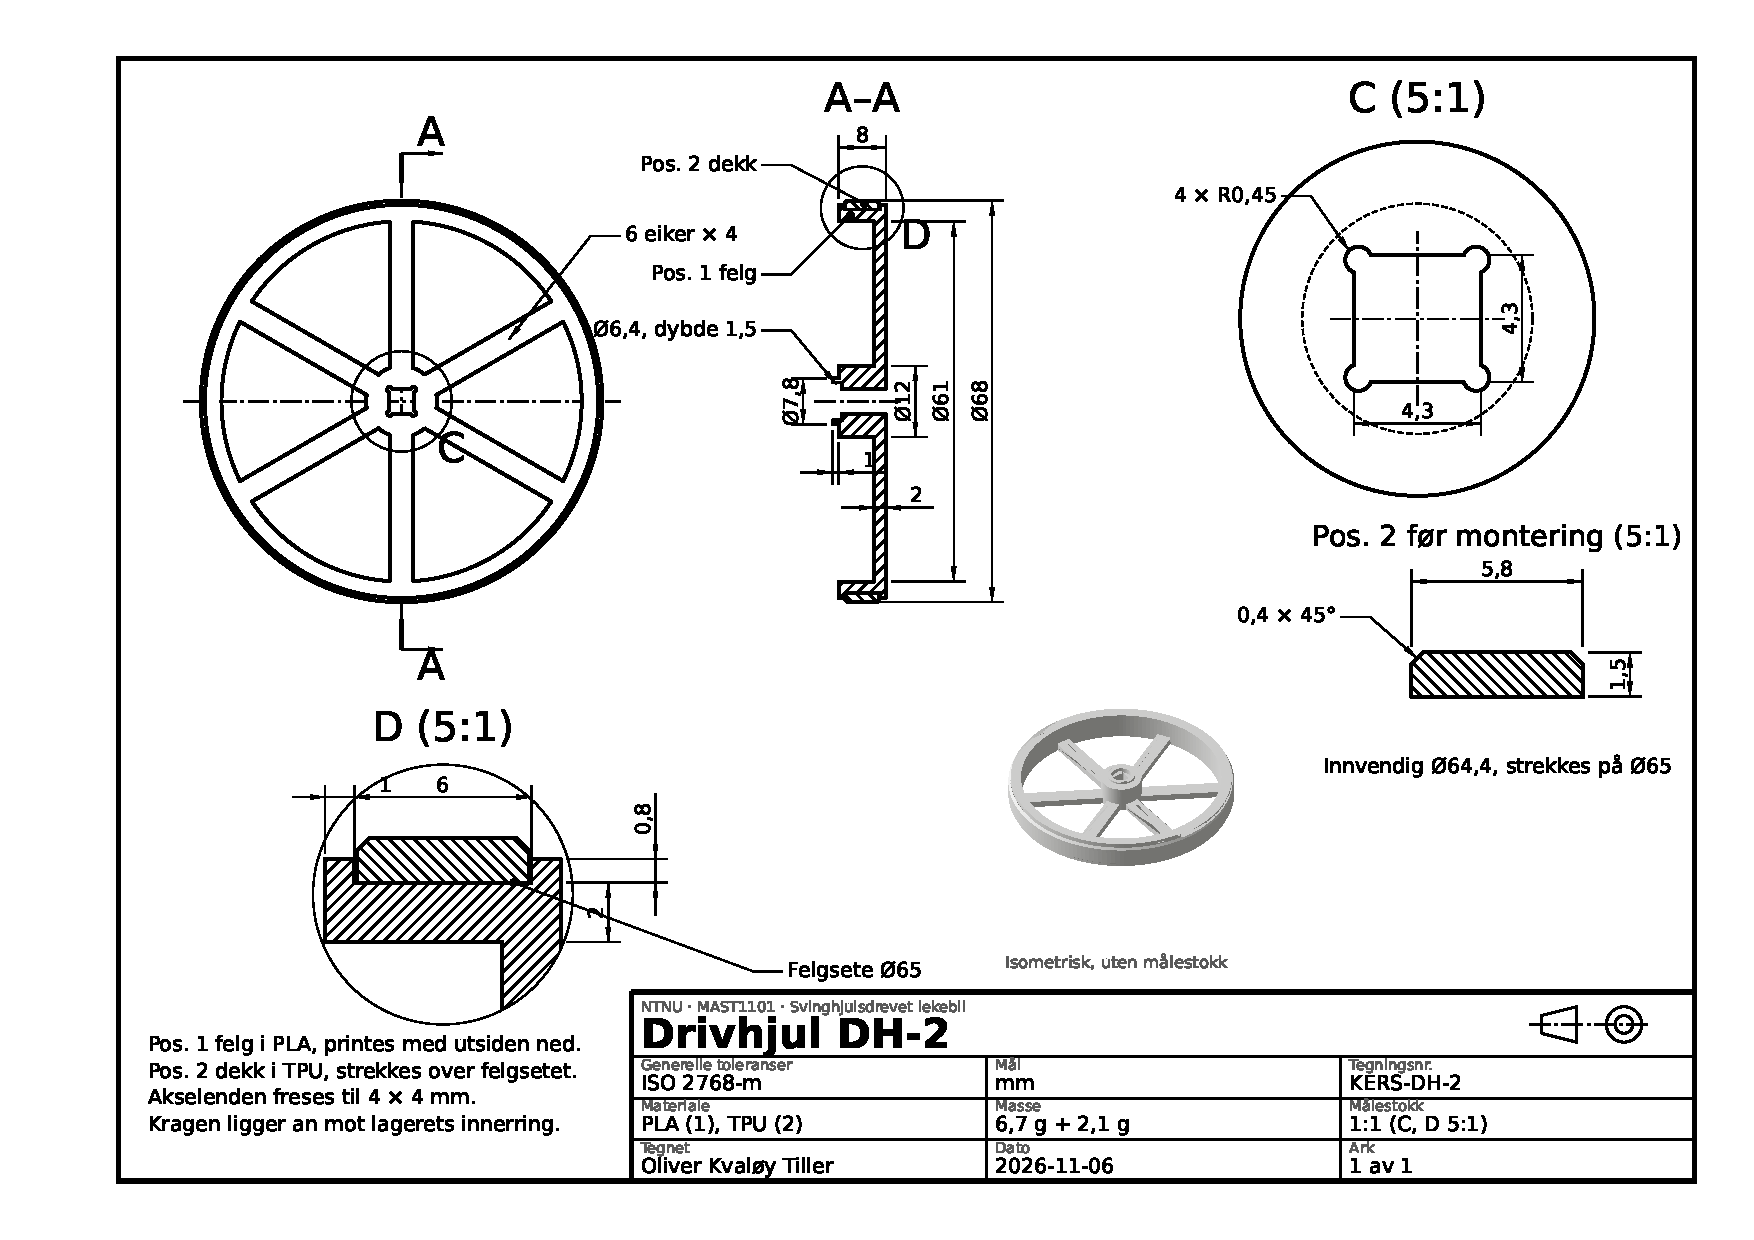
\includegraphics[width=\textheight]{Images/Tegninger/DH-2.pdf}
    \caption{Maskintegning av drivhjulet med felg (pos.~1) og TPU-dekk (pos.~2). Det bare hjulet har samme nav og eiker, men er et bart hjul med ytre diameter \SI{68}{mm}.}
    \label{fig:hjul}
\end{sidewaysfigure}

\clearpage
\subsection{Testprotokoll og rådata}
\label{app:raadata}
Utsnurringen per opptrekk for seriene i seksjon~\ref{sec:res-utsnurring}. Rådata ligger i \nolinkurl{Code/utsnurring_diagnose/data/}.

\begin{table}[H]
    \centering
    \caption{Utsnurring med tannhjulet koblet. Toppturtallet er rett etter at løkka slipper.}
    \label{tab:utsnurring-koblet}
    \small
    \renewcommand{\arraystretch}{1.3}
    \begin{tabular}{|c|c|c|c|c|}
        \hline
        \textbf{Opptrekk} & \textbf{Topp [o/min]} & \textbf{Til stopp [s]} & \textbf{1000 til 300 o/min [s]} & \textbf{Snittmoment [mN\,m]} \\
        \hline
        2 & 2166 & 3,88 & 1,66 & 2,66 \\
        3 & 2830 & 4,96 & 1,66 & 2,65 \\
        4 & 2281 & 4,20 & 1,61 & 2,74 \\
        6 & 3030 & 5,16 & 1,66 & 2,66 \\
        7 & 3125 & 4,76 & 1,56 & 2,83 \\
        8 & 2791 & 5,14 & 1,74 & 2,54 \\
        \hline
        \textbf{Snitt} & \textbf{2704 ± 394} & & \textbf{1,65 ± 0,06} & \textbf{2,68} \\
        \hline
    \end{tabular}
\end{table}

\begin{table}[H]
    \centering
    \caption{Utsnurring med tannhjulet frakoblet.}
    \label{tab:utsnurring-frakoblet}
    \small
    \renewcommand{\arraystretch}{1.3}
    \begin{tabular}{|c|c|c|c|c|}
        \hline
        \textbf{Opptrekk} & \textbf{Topp [o/min]} & \textbf{Til stopp [s]} & \textbf{1000 til 300 o/min [s]} & \textbf{Snittmoment [mN\,m]} \\
        \hline
        2 & 1709 & 6,97 & 3,27 & 1,35 \\
        3 & 1987 & 6,85 & 2,83 & 1,56 \\
        4 & 2362 & 5,56 & 2,40 & 1,83 \\
        5 & 2007 & 9,44 & 3,99 & 1,10 \\
        6 & 2335 & 5,65 & 2,17 & 2,03 \\
        \hline
        \textbf{Snitt} & \textbf{2080 ± 272} & & \textbf{2,93 ± 0,73} & \textbf{1,50} \\
        \hline
    \end{tabular}
\end{table}

\clearpage
\subsection{Bilder og dokumentasjon av prototypeversjoner}
